
\RequirePackage[pdf]{layout/hp-book}










\begin{document}
{
\pagestyle{empty}
\def\volumenumber{}
\def\volumetitle{Kapitel 1--\ref{last:chapter}} %  plus omake files 1--{4}
\newcommand{\fullvolumetitle}{\volumetitle}

\def\volumenumber{}
\def\volumetitle{Layout-Test vom \today{}}
\definecolor{gold}{rgb}{0.77,0.69,0.37}
\newlength{\hptitlewidth}
\newlength{\rationalh}
\newcommand{\hptitle}[2][\stockwidth]{%
\setlength{\hptitlewidth}{#1}%
\centering\color{white}%
\vskip 3cm\resizebox{.95\hptitlewidth}{!}{\textls[100]{HARRY POTTER AND THE}}%
\vskip 2mm%
\color{gold}%
\settoheight{\rationalh}{\resizebox{.95\hptitlewidth}{!}{\textls[20]{RATIONALITY}}}
\resizebox{!}{0.9\rationalh}{\textls[50]{METHODS}}%
\hfil\resizebox{!}{0.3\rationalh}{\textls[50]{Of}}%
\vskip 2mm%
\resizebox{.95\hptitlewidth}{!}{\textls[20]{RATIONALITY}}%
\vskip 8mm%
\color{white}%
\resizebox{.5\hptitlewidth}{!}{\textls[50]{\scshape{}Fanfiction von Eliezer Yudkowsky}}%
\vskip 4mm%
\resizebox{.35\hptitlewidth}{!}{\textls[50]{\scshape{}Deutsche Übersetzung}}%
\vfill%
\textls[50]{\scshape #2}%
\color{black}%
\vskip 1cm\ %
}
\providecommand{\fullvolumetitle}[1]{Buch #1: \volumetitle}

\ifcover%
\definecolor{backgroundcover}{HTML}{272c36}
\newpagecolor{backgroundcover}\afterpage{\restorepagecolor}
\newcommand\BackgroundPic{
\put(0,0){%
\parbox[b][\paperheight]{\paperwidth}{%
\vfill%
\centering%
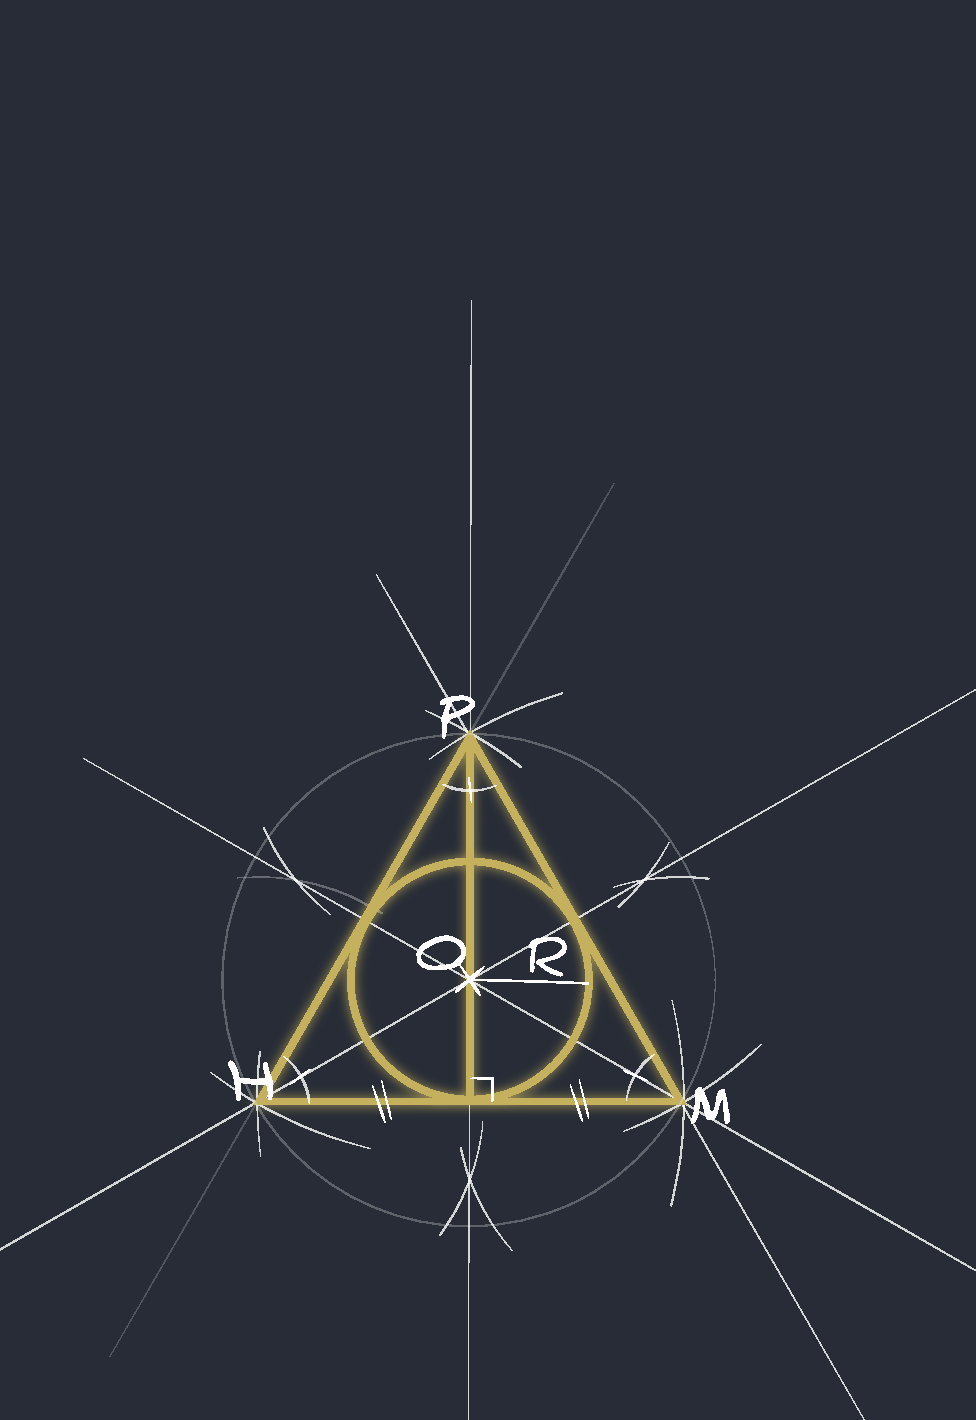
\includegraphics[width=\paperwidth,height=\paperheight,keepaspectratio]{images/cover1.pdf}%
\vfill%
}}}\AddToShipoutPicture*{\BackgroundPic}%
\AddToShipoutPicture*{\put(0,0){%
\parbox[b][\paperheight]{\paperwidth}{%
\hptitle{\fullvolumetitle{\volumenumber}}%
}}}%
\ %
\cleartorecto
\fi
\begin{center}
\thispagestyle{empty}
{\hpfont
\Huge\MakeUppercase{Harry Potter}\vspace*{0.5cm}

\Large\MakeUppercase{and the Methods of Rationality} %

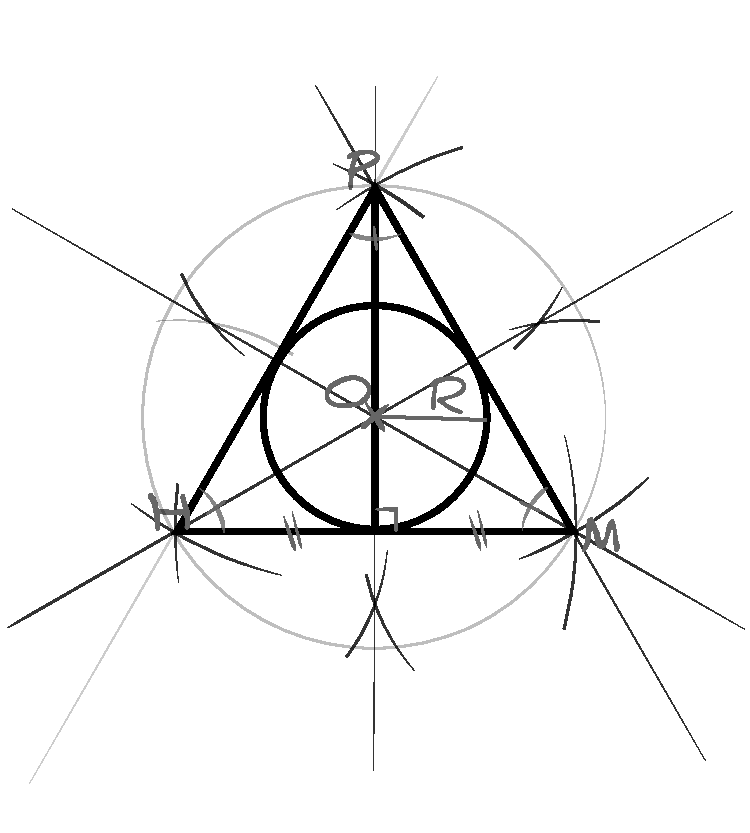
\includegraphics[scale=0.5]{images/bubble.pdf}

\vspace*{-1.0cm}
\Large Fanfiction von \vspace*{.25cm}

\huge \MakeUppercase{Eliezer Yudkowsky}%

\normalsize

\vspace*{1\baselineskip}
\fullvolumetitle{\volumenumber}
}

\vspace{0.7cm}

Basierend auf der Harry Potter Serie von J.~K.~Rowling\\
Author's disclaimer: J.~K.~Rowling owns Harry Potter, and no one owns the methods of rationality.
% Disclaimer: ~K.~Rowling besitzt alle Rechte an Harry Potter, aber niemandem gehören die Methods of Rationality.

~\\
Die englische Originalfassung gibt es auf {\small\url{http://hpmor.com}}\\
und auf {\small\url{https://github.com/rrthomas/hpmor/}} als überarbeites PDF und eBook.\\
\end{center}



\newpage
\vspace*{2cm}
\begin{center}
\noindent
Diese übersetzte Fassung ist ein \href{https://github.com/entorb/hpmor-de/}{OpenSource Projekt}\\
gestartet von \href{https://entorb.net}{Torben Menke}\\
{\small \url{https://github.com/entorb/hpmor-de/}}\\
\vspace*{3cm}
Mitarbeit und Verbesserungsvorschläge sind herzlich willkommen:\\
{\small\url{https://github.com/entorb/hpmor-de/wiki/Mitmachen}}\\
\vspace*{3cm}
Es werden diese Übersetzungen verwendet:\\
von Jost (Kapitel 1-21) {\small \url{https://www.fanfiktion.de/s/4cb8beb50000203e067007d0/}}\\
von Patneu (Kapitel 22-38) {\small \url{https://www.fanfiktion.de/s/55610c610004dede273a3811/}}\\
von DieFuechsin (Kapitel 39-78) {\small \url{https://www.fanfiktion.de/s/5c793dfe000a402030774dc7/}}\\
von Schneefl0cke (Kapitel 79-122) {\small \url{https://www.fanfiktion.de/s/60044849000ccc541aef297e/}}\\
\end{center}

% \chapter*{Content warnings}
\thispagestyle{empty}

Discussion (not depiction) of non-consensual sex: About 60\% of the way through Chapter 7; very briefly in an omake in Chapter 11.

First-person depiction (experienced by viewpoint character) of intense school bullying. Starting halfway through Chapter 19.

Violent character death. Chapter 89.

For more information (with spoilers!), see:
\begin{center}\url{https://wiki.lesswrong.com/wiki/MethodsOfRationality/TriggerWarnings}\end{center}

\pagenumbering{gobble}
\cleartorecto
\renewcommand*{\printtoctitle}[1]{\centering\Huge{\hpfont\MakeUppercase{#1}}}
\setlength{\cftbeforechapterskip}{.5\baselineskip plus 12pt minus 3pt}
\setlength{\cftbeforepartskip}{1\baselineskip plus 12pt minus 3pt}
\renewcommand*{\cftpartleader}{\space—\space}
\renewcommand*{\cftpartfillnum}[1]{%
 \cftpartafterpnum\par}
\renewcommand*{\cftchapterleader}{\space—\space}
\renewcommand*{\cftchapterfillnum}[1]{%
 {\cftchapterleader}\nobreak%
 {#1}%
 \cftchapterafterpnum\par}
\setrmarg{0em}
\setlength\cftpartindent{0pt}
\setlength\cftpartnumwidth{0pt}
\setlength\cftchapterindent{0pt}
\setlength\cftchapternumwidth{0pt}
\renewcommand*{\cftpartafterpnum}{\cftparfillskip}
\renewcommand*{\cftchapterafterpnum}{\cftparfillskip}
\renewcommand*{\cftpartfont}{}
\renewcommand*{\cftchapterfont}{}

\renewcommand\partnumberline[1]{\hfil\thispagestyle{empty}{\hpfont\textls[30]{\large\MakeUppercase{\partname} #1}}\hfil\strut\par\nopagebreak\hfil}
\renewcommand\chapternumberline[1]{\hfil\thispagestyle{empty}{\hpfont\textls[30]{\IfInteger{#1}{\NUMBERstringnum{#1}}{Appendix #1}}}\hfil\strut\par\nopagebreak\hfil}

\settocdepth{chapter}
\phantomsection
\label{contents}

\thispagestyle{empty}

\tableofcontents*

\clearpage
\thispagestyle{empty}
\hbox{}

% \makeatletter
\newlength{\beforeblurbskip}
  \setlength{\beforeblurbskip}{.5\baselineskip}
\newlength{\afterblurbskip}
  \setlength{\afterblurbskip}{.5\baselineskip}
\newlength{\blurbwidth}
  \setlength{\blurbwidth}{.6\textwidth}
\newlength{\blurbrule}
  \setlength{\blurbrule}{.4\p@}
\newcommand{\blurbsize}{\small}
\newcommand{\blurbflush}{flushright}

\newcommand{\blurbfontsize}[1]{\def\blurbsize{#1}}
\newcommand{\blurbposition}[1]{\long\def\blurbflush{#1}}
\newcommand{\blurbtextposition}[1]{\def\textflush{#1}}
\newcommand{\blurbsourceposition}[1]{\def\sourceflush{#1}}

\newcommand{\@blurbrule}{\rule[.5ex]{\blurbwidth}{\blurbrule}}

\newcommand{\@blurbtext}[1]{%
  \begin{minipage}{\blurbwidth}\begin{\textflush} #1\par
    \ifdim\blurbrule>\z@ \@blurbrule \else \vspace*{1ex} \fi
  \end{\textflush}\end{minipage}}

  \newcommand{\@blurbsource}[1]{%
  \begin{minipage}{\blurbwidth}
    \begin{\sourceflush} #1\par
  \end{\sourceflush}\end{minipage}}

\newcommand{\blurb}[2]{
	\vspace{\beforeblurbskip} 
	{\blurbsize
	\begin{\blurbflush}
		\begin{minipage}{8cm} \@blurbtext{#1}\\ \@blurbsource{#2} \end{minipage}
	\end{\blurbflush} 
	\vspace{\afterblurbskip}}}
\makeatother

\thispagestyle{empty}
\blurb{“[...A] terrific series, subtle and dramatic and stimulating.”}{David Brin}
\blurb{“Oh Thoth Trismegistus, oh Ma’at, oh Ganesha, oh sweet lady Eris… I have not laughed so hard in years!”}{Eric S. Raymond}
\thispagestyle{empty}

\cleartorecto
}
\pagenumbering{arabic}
\setcounter{page}{1}

\part{Layout Tests}


\chapter{Example Chapter ä-ö-ü-ß-Ä-Ö-Ü-SS}

\begin{chapterOpeningAuthorNote}
chapterOpeningAuthorNote: Every inch of wall space is covered by a bookcase. Each bookcase has six shelves, going almost to the ceiling.
\end{chapterOpeningAuthorNote}
\begin{chapterOpeningQuote}
chapterOpeningQuote: Other shelves have two layers of paperback science fiction, with the back layer of books propped up on old tissue boxes or lengths of wood, so that you can see the back layer of books above the books in front.
\end{chapterOpeningQuote}

\lettrine{E}{very} inch of wall space is covered by a bookcase. Each bookcase has six shelves, going almost to the ceiling. Some bookshelves are stacked to the brim with hardback books: science, maths, history, and everything else. Other shelves have two layers of paperback science fiction, with the back layer of books propped up on old tissue boxes or lengths of wood, so that you can see the back layer of books above the books in front. And it still isn’t enough. Books are overflowing onto the tables and the sofas and making little heaps under the windows.
ä-ö-ü-ß-Ä-Ö-Ü-SS

This is the living-room of the house occupied by the eminent Professor Michael Verres-Evans, and his wife, Mrs~Petunia Evans-Verres, and their adopted son, Harry James Potter-Evans-Verres. There is a letter lying on the living-room table, and an unstamped envelope of yellowish parchment, addressed to \emph{Mr~H.~Potter} in emerald-green ink.


\chapter{Font Styles ä-ö-ü-ß-Ä-Ö-Ü-SS}

\section{Basic Font Styles ä-ö-ü-ß-Ä-Ö-Ü-SS}

underline: \underline{underline ä-ö-ü-ß-Ä-Ö-Ü-SS}

textsc: \textsc{textsc ä-ö-ü-ß-Ä-Ö-Ü-SS}

textbf: \textbf{textbf ä-ö-ü-ß-Ä-Ö-Ü-SS}

emph: \emph{emph1 emph1 \emph{emph2 \emph{emph3} emph2} emph1 ä-ö-ü-ß-Ä-Ö-Ü-SS}

MakeUppercase: start \MakeUppercase{MakeUppercase ä-ö-ü-ß-Ä-Ö-Ü-SS} end

\section{tone of voice ä-ö-ü-ß-Ä-Ö-Ü-SS}

shout: \shout{shout shout ä-ö-ü-ß-Ä-Ö-Ü-SS}

scream: \scream{scream scream ä-ö-ü-ß-Ä-Ö-Ü-SS}

prophesy: \prophesy{prophesy prophesy ä-ö-ü-ß-Ä-Ö-Ü-SS}

parsel: \parsel{parsel parsel ä-ö-ü-ß-Ä-Ö-Ü-SS}

spell: \spell{spell spell ä-ö-ü-ß-Ä-Ö-Ü-SS}

abbrev: \abbrev{abbrev ä-ö-ü-ß-Ä-Ö-Ü-SS}

\section{abbreviations}
SPHEW: Start: \SPHEW.

\section{Newspaper}

1. healine: start \headline{my headline ä-ö-ü-ß-Ä-Ö-Ü-SS} end

2. inlineheadline: start \inlineheadline{my inline headline ä-ö-ü-ß-Ä-Ö-Ü-SS} end

3. healine env:
\begin{headlines}
my headline env ä-ö-ü-ß-Ä-Ö-Ü-SS
\end{headlines}
end

\section{special}
start McGonagallWhiteBoard: \McGonagallWhiteBoard{Hallo ä-ö-ü-ß-Ä-Ö-Ü-SS} end

translatorsnote:\translatorsnote{Translator's note is here ä-ö-ü-ß-Ä-Ö-Ü-SS. And it still isn’t enough. Books are overflowing onto the tables and the sofas and making little heaps under the windows.}

\section{writtenNote}
\begin{writtenNote}
\letterAddress{Sehr geehrte stellvertretende Schulleiterin ä-ö-ü-ß-Ä-Ö-Ü-SS}
And it still isn’t enough. Books are overflowing onto the tables and the sofas and making little heaps under the windows.

This is the living-room of the house occupied by the eminent Professor Michael Verres-Evans, and his wife, Mrs~Petunia Evans-Verres, and their adopted son, Harry James Potter-Evans-Verres. There is a letter lying on the living-room table, and an unstamped envelope of yellowish parchment, addressed to \emph{Mr~H.~Potter} in emerald-green ink.
\letterClosing[Mit freundlichen Grüßen]{Harry James Potter-Evans-Verres.}
\end{writtenNote}

\part{Doc Structure}

\partchapter{partchapter: The Stanford Prison Experiment}{I}
Text
This is the living-room of the house occupied by the eminent Professor Michael Verres-Evans, and his wife, Mrs~Petunia Evans-Verres, and their adopted son, Harry James Potter-Evans-Verres. There is a letter lying on the living-room table, and an unstamped envelope of yellowish parchment, addressed to \emph{Mr~H.~Potter} in emerald-green ink.

This is the living-room of the house occupied by the eminent Professor Michael Verres-Evans, and his wife, Mrs~Petunia Evans-Verres, and their adopted son, Harry James Potter-Evans-Verres. There is a letter lying on the living-room table, and an unstamped envelope of yellowish parchment, addressed to \emph{Mr~H.~Potter} in emerald-green ink.

\namedpartchapter{namedpartchapter: The Stanford Prison Experiment}{TSPE}{VI}{Constrained Optimization}
Text

later: text \later end later


\latersection{latersection ä-ö-ü-ß-Ä-Ö-Ü-SS}
start latersection









\end{document}
